\section{紧算子}
\label{sec:lop-compact}

有界算子把有界输入变成有界输出，但无限维空间中有界序列未必有收敛子列，所以有界性本身不保证输出能被有限多个代表近似。本节要求有界输入列的输出能选出范数收敛的子列，由此得到比有界性更强的紧性。我们先比较有限秩算子与无限维恒等算子，再在Hilbert空间中建立有限秩逼近，最后把结论用于平方可积核的积分算子。

\subsection{紧算子的定义}
\label{sec:lop-compact-def}

第~\ref{chap:topological-spaces}章把闭包紧的集合称为相对紧集；第~\ref{chap:metric-spaces}章说明，在度量空间中，集合相对紧当且仅当其中每个序列都有在全空间中收敛的子列，并且在完备度量空间中这又等价于全有界，即对每个$\varepsilon>0$都能被有限个半径$\varepsilon$的球覆盖。下面把这一性质加在算子的像上。

先看输出落在有限维空间中的情形。有界线性算子$F:X\to Y$若像$\operatorname{Ran}F$是有限维子空间，就称为\term{有限秩算子}（finite-rank operator），$\dim\operatorname{Ran}F$称为它的秩。若$\lVert x_n\rVert\leq C$，则$\lVert Fx_n\rVert\leq\lVert F\rVert C$，输出序列落在有限维空间的一个有界集合中。有限维赋范空间中所有范数等价，有界序列总有收敛子列，所以$(Fx_n)$有范数收敛的子列。

\begin{definition}[紧算子]
\label{def:lop-compact-operator}
设$X,Y$是赋范空间，$T:X\to Y$是线性算子。若$X$的闭单位球$B_X$的像$T(B_X)$在$Y$中相对紧，则称$T$为\term{紧算子}（compact operator）。等价地，对$X$中每个有界序列$(x_n)$，输出序列$(Tx_n)$都有在$Y$中按范数收敛的子列。
\end{definition}

两种说法等价，是因为有界序列经缩放后落在某个$rB_X$中，而$T(rB_X)=rT(B_X)$与$T(B_X)$同时相对紧。紧算子必然有界：若$T$无界，可取单位向量$x_n$使$\lVert Tx_n\rVert\geq n$，输出序列的任何子列都无界，不可能收敛。由上一段，每个有界有限秩算子都是紧算子。

\paragraph{无限维恒等算子不紧}
紧性不是每个有界算子都具备的。设$H$是无限维Hilbert空间，取标准正交序列$(e_n)$。对$n\neq m$，$\lVert e_n-e_m\rVert^2=\lVert e_n\rVert^2+\lVert e_m\rVert^2=2$。恒等算子$I$把这个有界序列原样输出，任意两项相距$\sqrt2$，没有柯西子列，因而没有收敛子列，$I$不是紧算子。一般的无限维赋范空间中，第~\ref{chap:functions-as-vectors}章用Riesz引理说明闭单位球不紧，所以恒等算子同样不紧。

同一个序列经过$\ell^2$上的对角算子$A(x_n)=(x_n/n)$后变成$Ae_n=e_n/n$，按范数趋于零。图~\ref{fig:lop-identity-orthonormal}比较了两种输出。$A$的单位球像满足$\lvert(Ax)_n\rvert\leq1/n$，越靠后的方向被压得越扁；下一小节将用有限秩逼近证明它是紧算子。

\begin{figure}[!htb]
  \centering
  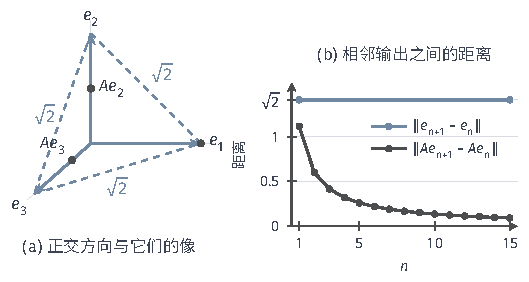
\includegraphics[width=89.6mm]{figures/02-abstract-mathematics/03-function-spaces/tikz/c3-identity-orthonormal/figure.pdf}
  \caption{同一个标准正交序列经过恒等算子与经过$A(x_n)=(x_n/n)$的对比。(a)~$e_1,e_2,e_3$两两相距$\sqrt2$（虚线），它们在$A$下的像$e_1$、$e_2/2$、$e_3/3$（黑点）向原点收拢；(b)~相邻输出的距离在恒等算子下恒为$\sqrt2$，在$A$下等于$\sqrt{1/n^2+1/(n+1)^2}$并趋于零。}
  \label{fig:lop-identity-orthonormal}
\end{figure}

这个例子说明紧性约束的对象。每个$x\in H$都能被它在前$n$个基向量上的截断任意逼近，单独看每个元素，有限截断都可行；紧性要求的却是同一个算子作用于整个有界输入族之后，输出整体可以被有限个代表覆盖。恒等算子对每个输入都能截断，对整个单位球却不能。

\paragraph{弱收敛的输入与范数收敛的输出}
第~\ref{chap:linear-functionals}章的标准正交序列满足$e_n\rightharpoonup0$而不按范数收敛。上例中$Ae_n=e_n/n$却按范数收敛到$A0=0$。这不是巧合：紧算子把弱收敛的输入变成范数收敛的输出。需要区分的是，弱收敛是输入列在全部连续线性观测下的收敛，相对紧是输出集合在范数距离下的性质，定理说明紧性在二者之间架起桥梁。

\begin{theorem}[紧算子改善收敛]
\label{thm:lop-compact-weak-strong}
设$X,Y$是赋范空间，$T:X\to Y$是紧算子。若$x_n\rightharpoonup x$，则$\lVert Tx_n-Tx\rVert\to0$。
\end{theorem}

\begin{proof}
第一步，输出弱收敛。对每个$\ell\in Y^*$，复合$\ell\circ T$是$X$上的有界线性泛函，所以$\ell(Tx_n)\to\ell(Tx)$，即$Tx_n\rightharpoonup Tx$。这一步只用到$T$有界。

第二步，反证。假设$Tx_n$不按范数收敛到$Tx$，则存在$\varepsilon>0$及子列$(x_{n_k})$，使$\lVert Tx_{n_k}-Tx\rVert\geq\varepsilon$对一切$k$成立。由第~\ref{chap:linear-functionals}章，弱收敛序列有界，所以$(x_{n_k})$有界；由紧性，可以再抽出子列，使相应的输出按范数收敛到某个$y\in Y$。

第三步，确认极限。范数收敛蕴含弱收敛，所以沿这个更细的子列，输出同时弱收敛到$y$和$Tx$。连续线性泛函能区分$Y$中不同的点（第~\ref{chap:linear-functionals}章由Hahn--Banach定理得到），弱极限唯一，故$y=Tx$。这与$\lVert Tx_{n_k}-Tx\rVert\geq\varepsilon$矛盾。
\end{proof}

对一般有界算子，第二步不成立：恒等算子把$e_n\rightharpoonup0$原样输出，输出仍只是弱收敛。

\subsection{Hilbert空间中的有限秩逼近}
\label{sec:lop-finite-rank-approx}

上面的例子提示，紧算子可以看成有限秩算子的极限。这里有两个方向：有限秩算子的算子范数极限是否紧，以及紧算子能否由有限秩算子按算子范数逼近。第一个方向在任意Banach取值空间中成立；第二个方向我们在Hilbert空间中证明。

\begin{theorem}[算子范数极限保持紧性]
\label{thm:lop-compact-limit}
设$X$是赋范空间，$Y$是Banach空间，$T_n:X\to Y$都是紧算子，$T\in\mathcal B(X,Y)$且$\lVert T_n-T\rVert\to0$。则$T$是紧算子。
\end{theorem}

\begin{proof}
$Y$完备，所以只需证明$T(B_X)$全有界：全有界集合的闭包仍全有界，又作为完备空间的闭子集完备，因而是紧集。给定$\varepsilon>0$，先取$n$使$\lVert T_n-T\rVert<\varepsilon$。$T_n(B_X)$相对紧，因而全有界，存在有限个点$y_1,\ldots,y_N\in Y$，使每个$T_nx$（$x\in B_X$）都与某个$y_i$相距小于$\varepsilon$。

对任意$x\in B_X$，选出相应的$y_i$，用三角不等式把误差拆成两段：
\[
\lVert Tx-y_i\rVert\leq\lVert(T-T_n)x\rVert+\lVert T_nx-y_i\rVert<\lVert T-T_n\rVert+\varepsilon<2\varepsilon .
\]
所以同一组$y_1,\ldots,y_N$是$T(B_X)$的有限$2\varepsilon$网。$\varepsilon$任意，$T(B_X)$全有界。
\end{proof}

关键在于误差界$\lVert T-T_n\rVert$对单位球中的全部输入同时成立，$T_n$的有限覆盖才能整体搬给$T$。若只知道$T_nx\to Tx$对每个$x$成立，就无法这样搬运：第~\ref{sec:lop-operator-convergence}节的截断投影$P_n$强算子收敛到$I$，每个$P_n$都是有限秩的，极限$I$却不紧。

\begin{example}[对角算子的有限秩逼近]
\label{ex:lop-diagonal-finite-rank}
在$\ell^2$上令$A(x_n)=(x_n/n)$，并令$A_m$只保留前$m$个坐标：$A_mx=(x_1,x_2/2,\ldots,x_m/m,0,0,\ldots)$，它的像落在前$m$个坐标张成的空间中，是有限秩算子。差$(A-A_m)x$只剩第$m+1$个坐标以后的部分，
\[
\lVert(A-A_m)x\rVert^2=\sum_{n>m}\frac{\lvert x_n\rvert^2}{n^2}\leq\frac{1}{(m+1)^2}\sum_{n>m}\lvert x_n\rvert^2\leq\frac{\lVert x\rVert^2}{(m+1)^2},
\]
取$x=e_{m+1}$时等号成立，所以$\lVert A-A_m\rVert=1/(m+1)\to0$。由定理~\ref{thm:lop-compact-limit}，$A$是紧算子。
\end{example}

图~\ref{fig:lop-finite-rank-error}把这个误差与恒等算子的截断比较。用$P_m$逼近恒等算子时，统一误差$\lVert I-P_m\rVert$恒为$1$；对固定的$x$，误差$\lVert(I-P_m)x\rVert$趋于零，但速度依赖$x$。对角算子的截断误差则按$1/(m+1)$对全部单位输入同时下降。

\begin{figure}[!htb]
  \centering
  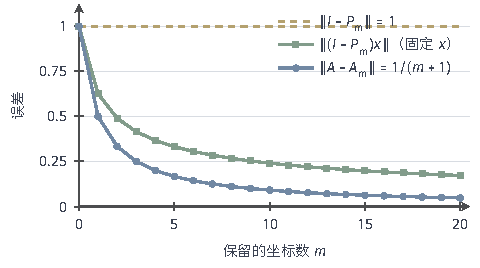
\includegraphics[width=81.2mm]{figures/02-abstract-mathematics/03-function-spaces/tikz/c3-finite-rank-error/figure.pdf}
  \caption{$\ell^2$上三种截断误差随保留坐标数$m$的变化。虚线：恒等算子的统一误差$\lVert I-P_m\rVert$恒为$1$。方点：固定单位向量$x\propto(1/n)$的误差$\lVert(I-P_m)x\rVert$趋于零，但这一速度只属于这个$x$。圆点：紧算子$A(x_n)=(x_n/n)$的统一误差$\lVert A-A_m\rVert=1/(m+1)$。}
  \label{fig:lop-finite-rank-error}
\end{figure}

\paragraph{紧算子的有限秩逼近}
现在证明反方向。思路是：紧算子的单位球像可以被有限个点以误差$\varepsilon$覆盖，这些点张成一个有限维子空间；向这个子空间作正交投影，就得到有限秩近似。正交投影的最近点性质保证投影误差不超过到覆盖点的距离。

\begin{theorem}[紧算子的有限秩逼近]
\label{thm:lop-finite-rank-approx}
设$X$是赋范空间，$H$是Hilbert空间，$T:X\to H$是紧算子。则存在有限秩算子$F_n:X\to H$，使$\lVert T-F_n\rVert\to0$。
\end{theorem}

\begin{proof}
给定$\varepsilon>0$。$T(B_X)$相对紧，因而全有界，取有限个点$y_1,\ldots,y_N$构成它的$\varepsilon$网。令$M=\operatorname{span}\{y_1,\ldots,y_N\}$，它是有限维子空间，因而闭；设$P$为到$M$的正交投影，令$F=PT$。$F$的像含于$M$，且$\lVert F\rVert\leq\lVert P\rVert\,\lVert T\rVert\leq\lVert T\rVert$，所以$F$是有界有限秩算子。

对任意$x\in B_X$，选$y_i$使$\lVert Tx-y_i\rVert<\varepsilon$。$PTx$是$M$中离$Tx$最近的点，而$y_i\in M$，所以
\[
\lVert Tx-Fx\rVert=\lVert Tx-PTx\rVert\leq\lVert Tx-y_i\rVert<\varepsilon .
\]
对$x\in B_X$取上确界得$\lVert T-F\rVert\leq\varepsilon$。令$\varepsilon=1/n$即得所需的算子列。
\end{proof}

这里控制的是整个单位球上的算子范数误差$\lVert T-F\rVert$，而不是只让$F$在有限几个输入上与$T$吻合；后者用强算子收敛就能做到，却不能保证统一误差。结合两个定理，在取值空间为Hilbert空间时，紧算子恰好是有界有限秩算子的算子范数极限。

证明真正用到的是Hilbert空间的正交投影：它把有限覆盖变成一个范数不超过$1$的线性“取最近点”操作。一般Banach空间中，有限维子空间上不一定有范数可控的投影族，紧算子能否由有限秩算子按算子范数逼近取决于空间的所谓逼近性质；确实存在不具有这一性质的Banach空间，这里不给出构造。所以本定理不能无条件推广，而定理~\ref{thm:lop-compact-limit}的方向在Banach空间中始终成立。

\subsection{积分算子的紧性}
\label{sec:lop-integral-compact}

沿用第~\ref{sec:lop-integral-bounded}小节的设定：$(X,\mu)$与$(Y,\nu)$是$\sigma$有限测度空间，$k\in L^2(X\times Y,\mu\otimes\nu)$，$T:L^2(Y,\nu)\to L^2(X,\mu)$由\eqref{eq:lop-integral-operator}给出。式\eqref{eq:lop-hs-norm}的估计对任意平方可积核成立，用于两个核之差就得到
\begin{equation}
\lVert T_k-T_{k^\prime}\rVert\leq\lVert k-k^\prime\rVert_{L^2(\mu\otimes\nu)},
\label{eq:lop-kernel-error}
\end{equation}
其中$T_k$表示以$k$为核的积分算子。所以只需用“给出有限秩算子的核”在$L^2$中逼近$k$，再用定理~\ref{thm:lop-compact-limit}。

\paragraph{分离变量的核给出有限秩算子}
若$k(x,y)=\sum_{i=1}^r\varphi_i(x)\psi_i(y)$，其中$\varphi_i\in L^2(\mu)$、$\psi_i\in L^2(\nu)$，则
\[
(Tf)(x)=\sum_{i=1}^r\Bigl(\int_Y\psi_i f\,\mathrm d\nu\Bigr)\varphi_i(x),
\]
输出落在$\operatorname{span}\{\varphi_1,\ldots,\varphi_r\}$中，$T$的秩不超过$r$。贯穿例子的核$1+xz=1\cdot1+x\cdot z$就是这样的有限和，所以\eqref{eq:lop-running-kernel}是秩为$2$的算子。最简单的分离变量核是可测矩形的示性函数$\mathbf 1_{A\times B}(x,y)=\mathbf 1_A(x)\mathbf 1_B(y)$，下面的引理说明它们的线性组合足以逼近任意可测集。

\begin{lemma}[矩形逼近]
\label{lem:lop-rectangle-approx}
设$(X,\mu)$、$(Y,\nu)$是有限测度空间，$E$属于乘积$\sigma$代数。则对每个$\varepsilon>0$，存在有限个两两不交的可测矩形，其并$R$满足$(\mu\otimes\nu)(E\,\triangle\,R)<\varepsilon$。
\end{lemma}

\begin{proof}
记$m=\mu\otimes\nu$，令$\mathcal E$为具有引理性质的可测集全体，$\mathcal R$为有限个两两不交可测矩形之并组成的族。两个矩形之交仍是矩形，矩形的补$(A\times B)^c=(A^c\times Y)\cup(A\times B^c)$是两个不交矩形之并，由此可知$\mathcal R$对有限交、补和有限并封闭。可测矩形显然属于$\mathcal E$。

若$E\in\mathcal E$，取$R\in\mathcal R$逼近它，则$R^c\in\mathcal R$且$E^c\triangle R^c=E\triangle R$，所以$\mathcal E$对补封闭。若$E_1,E_2,\ldots\in\mathcal E$，令$E=\bigcup_jE_j$。总测度有限，可取$N$使$m(E\setminus\bigcup_{j\leq N}E_j)<\varepsilon/2$；再对$j\leq N$取$R_j\in\mathcal R$使$m(E_j\triangle R_j)<\varepsilon/(2N)$。令$R=\bigcup_{j\leq N}R_j\in\mathcal R$，则
\[
m(E\triangle R)\leq m\Bigl(E\setminus\bigcup_{j\leq N}E_j\Bigr)+\sum_{j\leq N}m(E_j\triangle R_j)<\varepsilon .
\]
所以$\mathcal E$对可数并封闭。$\mathcal E$是包含全部可测矩形的$\sigma$代数，因而包含它们生成的乘积$\sigma$代数。
\end{proof}

\begin{theorem}[矩形阶梯核的稠密性]
\label{thm:lop-rectangle-dense}
形如
\begin{equation*}
\sum_{i=1}^rc_i\mathbf 1_{A_i}(x)\mathbf 1_{B_i}(y)\qquad(\mu(A_i),\nu(B_i)<\infty)
\end{equation*}
的函数在$L^2(X\times Y,\mu\otimes\nu)$中稠密。
\end{theorem}

\begin{proof}
第一步，截断到有限测度区域。由$\sigma$有限性，取递增的可测集$X_j\uparrow X$、$Y_j\uparrow Y$，且$\mu(X_j),\nu(Y_j)<\infty$。令$k_j=k\mathbf 1_{X_j\times Y_j}$，则$\lvert k-k_j\rvert^2\leq\lvert k\rvert^2$且逐点趋于零，由控制收敛定理$\lVert k-k_j\rVert_{L^2}\to0$。

第二步，用简单函数逼近。对$k_j$取简单函数$s_n\to k_j$逐点收敛且$\lvert s_n\rvert\leq\lvert k_j\rvert$（实部、虚部分别取单调逼近），则$\lvert k_j-s_n\rvert^2\leq4\lvert k_j\rvert^2$，由控制收敛定理$\lVert k_j-s_n\rVert_{L^2}\to0$。每个$s_n$是有限个$c_i\mathbf 1_{E_i}$之和，$E_i\subseteq X_j\times Y_j$可测。

第三步，用矩形代替可测集。在有限测度空间$X_j$与$Y_j$上应用引理~\ref{lem:lop-rectangle-approx}，每个$E_i$都可被有限个不交矩形之并$R_i$逼近，且$\lVert\mathbf 1_{E_i}-\mathbf 1_{R_i}\rVert_{L^2}=m(E_i\triangle R_i)^{1/2}$可任意小。三步的误差相加即得结论。
\end{proof}

\begin{theorem}[平方可积核给出紧算子]
\label{thm:lop-hs-compact}
在本小节的设定下，$T:L^2(Y,\nu)\to L^2(X,\mu)$是紧算子。
\end{theorem}

\begin{proof}
由定理~\ref{thm:lop-rectangle-dense}，对每个$\varepsilon>0$存在$k_\varepsilon(x,y)=\sum_{i=1}^rc_i\mathbf 1_{A_i}(x)\mathbf 1_{B_i}(y)$使$\lVert k-k_\varepsilon\rVert_{L^2}<\varepsilon$。$k_\varepsilon$是分离变量核，对应的积分算子把$f$送到$\sum_ic_i\bigl(\int_{B_i}f\,\mathrm d\nu\bigr)\mathbf 1_{A_i}$，是有限秩算子。由\eqref{eq:lop-kernel-error}，算子范数误差不超过$\varepsilon$。$L^2(X,\mu)$完备，由定理~\ref{thm:lop-compact-limit}，$T$是紧算子。
\end{proof}

证明中出现两种误差。$\lVert k-k_\varepsilon\rVert_{L^2(\mu\otimes\nu)}$度量的是两个核函数在乘积空间上的平方积分差，$\lVert T-T_{k_\varepsilon}\rVert$度量的是两个算子对单位输入的最坏输出差。式\eqref{eq:lop-kernel-error}只给出前者控制后者的单向关系；后者可以严格更小，正如贯穿例子中$\lVert T\rVert=1<\lVert k\rVert_{L^2}$。

图~\ref{fig:lop-rectangle-kernel}在贯穿例子上演示这一逼近。用$n\times n$网格上的格内平均作分片常数核$k_n$，它是$n^2$个矩形示性函数的线性组合，误差$\lVert k-k_n\rVert_{L^2}$大致按$1/n$下降。对这个核，分片常数逼近远不是最经济的：$k$本身的秩为$2$，两项就精确。矩形逼近的价值在于它对任意平方可积核都可行，从而在不知道核的任何具体结构时证明了紧性；按奇异值选取最经济的有限秩近似，是第~\ref{chap:operator-spectra}章的问题。

\begin{figure}[!htb]
  \centering
  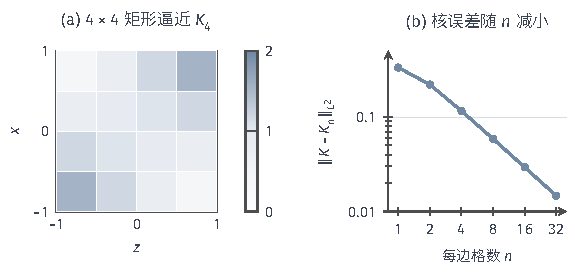
\includegraphics[width=97.4mm]{figures/02-abstract-mathematics/03-function-spaces/tikz/c3-rectangle-kernel/figure.pdf}
  \caption{用矩形示性函数的线性组合逼近核$k(x,z)=1+xz$（乘积测度由$\mathrm dz/2$给出）。(a)~$4\times4$均匀网格上取格内平均得到的分片常数核，每格对应一个可测矩形；(b)~$n\times n$网格平均的误差$\lVert k-k_n\rVert_{L^2}$，从$n=1$时的$1/3$降到$n=32$时约$0.015$，大致按$1/n$下降；它同时是相应有限秩算子的算子范数误差上界。}
  \label{fig:lop-rectangle-kernel}
\end{figure}
